\documentclass[10pt]{article}
\usepackage{icmlko}

\icmlmeta{IP 파운데이션 월드모델}{238}{같은 처방이 도메인마다 다르게 듣는다}{노트 237의 문턱 해제를 모바일에도 했다. 덮음은 같은 폭으로 올랐는데 도메인 rho 는 게임만 오른다}

\begin{document}

\twocolumn[
\icmlheader

\begin{abstract}
노트 237이 \texttt{MIN\_HANGUL} 문턱을 떼고 게임 영문 195건을 받아
\textbf{덮음 24.4\% $\to$ 56.7\% · 게임 $\rho$ $+$0.0221 · F21
$+$0.0027($t{=}2.37$)} 을 얻었다. 같은 처방을 모바일에 했다.
\textbf{덮음은 같은 폭으로 오르는데}(34.9\% $\to$ 62.8\%, $+$28\%p)
\textbf{도메인 $\rho$ 가 안 움직인다}($+$0.5283 $\to$ $+$0.5276) 그리고
판도 F21 $+$0.0021($t{=}0.61$) · F23 $+$0.0008($t{=}0.27$)로 유의하지
않다. 갈랐다. \textbf{까닭은 새 축이 기존 축보다 센가에 있다} ---
게임에서 영문 질의의 level$\leftrightarrow$라벨이 \textbf{$+$0.480} 이고
한글 질의가 $+$0.381 이라 \emph{채울수록 도메인 평균이 올라간다.} 모바일은
반대다 --- 영문 $+$0.348 · 한글 $+$0.501 이라 \textbf{채울수록 희석된다.}
검색량 자체도 다르다(level 중앙 게임 영문 0.0141 · 모바일 영문 0.0068).
읽으면 그럴듯하다 --- \textbf{스팀 게임은 한국에서도 영문명으로 찾고}
(``Counter-Strike'' 를 ``카운터 스트라이크''보다 많이 친다)
\textbf{모바일 영문 제목은 이름 없는 인디 앱이라 아무 이름으로도 안
찾는다.} 그래서 규칙이 하나 나온다: \textbf{덮음을 채울 때는 채우는 축이
이미 있는 축보다 센지 먼저 봐야 한다.} 세면 도메인이 오르고, 약하면
덮음만 오르고 $\rho$ 는 제자리다 --- \textbf{그리고 그것은 유보를 안 보고
잴 수 있다}(학습 구간에서 두 질의 방식의 상관을 견주면 된다). 그래도
모바일 것을 안 물린다 --- \textbf{해롭지 않고}(F18 $-$0.0003 · $t{=}-0.14$)
\textbf{덮음은 진짜로 올랐으며}, 노트 234가 잰 대로 대입 행이 관측 행보다
$\rho$ 가 낮으므로 채운 것 자체가 자료의 개선이다. 이 사이클의 누적은
F23 $+$0.4524 $\to$ $+$0.4546 이다.
\end{abstract}
]

\begin{figure*}[t]
\centering
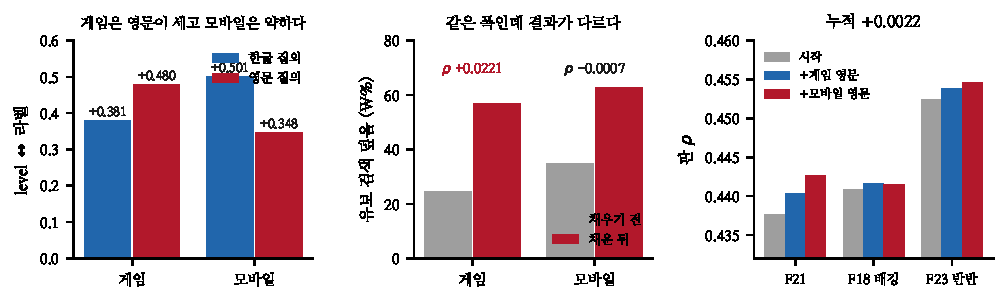
\includegraphics[width=\textwidth]{figs/samefix.pdf}
\caption{왼쪽 --- 게임은 영문이 세고 모바일은 약하다. 가운데 --- 같은
폭인데 결과가 다르다. 오른쪽 --- 누적 $+$0.0022.}
\end{figure*}

\section{같은 폭, 다른 결과}

\begin{table}[t]
\centering\tsize
\caption{문턱 해제 뒤.}
\begin{tabular}{lrrrr}
\toprule
& 덮음 전 & 덮음 후 & 도메인 $\rho$ & $t$(F21) \\
\midrule
\textbf{게임} & 24.4\% & 56.7\% & \textbf{$+$.0221} & \textbf{2.37} \\
모바일 & 34.9\% & 62.8\% & $-$.0007 & 0.61 \\
\bottomrule
\end{tabular}
\end{table}

\claimx{\textbf{덮음은 같은 폭으로 오르는데}($+$32\%p 대 $+$28\%p)
\textbf{도메인 $\rho$ 는 게임만 오른다.}}{모바일 짝검정도 유의하지 않다
--- F21 $+$0.0021($t{=}0.61$) · F18 $-$0.0003($t{=}-0.14$) · F23
$+$0.0008($t{=}0.27$).}

\claimx{\textbf{그리고 앞서 적은 덮음 수가 틀렸다} --- ``60.1\% $\to$
62.8\%''로 읽었는데 60.1\% 는 노트 221 시점 값이고, 그 뒤 노트 222의
계열 질의 마스크가 실효 덮음을 낮췄다. \textbf{실제로는 34.9\% $\to$
62.8\%} 다.}{판정치 옆에 덮음을 적기 시작한 것이 노트 231인데,
\textbf{덮음 자체도 어느 시점 어느 마스크에서 잰 것인지 적어야 한다.}}

\section{새 축이 기존 축보다 센가}

\begin{table}[t]
\centering\tsize
\caption{level $\leftrightarrow$ 라벨(관측된 행만).}
\begin{tabular}{lrrr}
\toprule
& 한글 질의 & 영문 질의 & level 중앙(영문) \\
\midrule
\textbf{게임} & $+$.381 & \textbf{$+$.480} & .0141 \\
\textbf{모바일} & \textbf{$+$.501} & $+$.348 & .0068 \\
\bottomrule
\end{tabular}
\end{table}

\claimx{\textbf{게임은 영문 질의가 한글보다 세고}($+$0.480 대 $+$0.381)
\textbf{모바일은 약하다}($+$0.348 대 $+$0.501). 채울수록 게임은 평균이
오르고 모바일은 희석된다.}{\textbf{읽으면 그럴듯하다} --- 스팀 게임은
한국에서도 영문명으로 찾고, 모바일 영문 제목은 이름 없는 인디 앱이라
아무 이름으로도 안 찾는다(검색량 중앙이 게임의 절반이다).}

\claimx{\textbf{규칙 하나가 나온다: 덮음을 채울 때는 채우는 축이 이미
있는 축보다 센지 먼저 봐야 한다.}}{\textbf{그리고 그것은 유보를 안 보고
잴 수 있다} --- 학습 구간에서 두 질의 방식의 축$\leftrightarrow$라벨을
견주면 된다. \textbf{노트 220의 천장표가 ``이 무리가 얼마짜리냐''를
줬다면 이것은 ``이 채움이 그 무리를 세게 하냐''를 준다.}}

\section{그래도 안 물린다}

\claimx{\textbf{모바일 것을 안 물린다} --- 해롭지 않고(F18 $-$0.0003 ·
$t{=}-0.14$) 덮음은 진짜로 올랐다.}{\textbf{노트 234가 잰 대로 대입 행이
관측 행보다 $\rho$ 가 낮으므로}(모바일 $+$0.21) \textbf{채운 것 자체가
자료의 개선이다} --- 판이 지금 안 움직이는 것은 새 축이 약해서지 자료가
나빠져서가 아니다.}

\claimx{\textbf{노트 236과 다른 판단이다.} 거기서는 채운 216건을 물렸다 ---
\emph{같은 축 값을 다른 라벨에 붙이는} 것이라 순위를 못 만들었기
때문이다.}{여기서는 \emph{각 레코드가 자기 질의의 값}을 받는다 ---
약할 뿐 틀리지 않았다. \textbf{``약한 참''과 ``틀린 값''을 가르는 것이
이 두 노트의 차이다.}}

\begin{table}[t]
\centering\tsize
\caption{이 사이클의 검색 축 작업.}
\begin{tabular}{lrl}
\toprule
& F23 & \\
\midrule
시작 & .4524 & \\
$+$게임 영문 195 & .4538 & 게임 $\rho$ $+$.0221 \\
$+$모바일 영문 203 & \textbf{.4546} & 모바일 $\rho$ 제자리 \\
\bottomrule
\end{tabular}
\end{table}

\begin{table}[t]
\centering\tsize
\caption{남은 것.}
\begin{tabular}{ll}
\toprule
\textbf{센가 먼저} & 채우기 전 두 질의를 견주는 절차 \\
\textbf{2016 이전} & 405건 --- 데이터랩 소급 한계 \\
덮음의 시점 & 덮음도 언제 어느 마스크인지 적을 것 \\
\bottomrule
\end{tabular}
\end{table}

첫 줄이 값싸고 이 노트를 규약으로 만든다. \textbf{채우기 전에 학습
구간에서 ``새 질의 방식의 축이 기존 것보다 센가''를 재면, 게임은 하고
모바일은 미룰 수 있었다.} 이번에는 둘 다 하고 나서 알았고 비용은
요청 230회였다 --- 크지 않지만 \textbf{이 사이클에서 천장표(노트 220) ·
도메인 천장(222) · 덮음 보고(231)를 세운 것과 같은 성질의 절차이고,
그 셋이 다 ``재기 전에 알 수 있는 것''이었다.} 네 번째를 추가한다:
\textbf{채우기 전에 채울 것의 세기를 재라.}

\end{document}
